%This is a LaTeX template for homework assignments
\documentclass{article}
\usepackage[utf8]{inputenc}
\usepackage{amsmath}
\usepackage{graphicx}
\usepackage{float}
\usepackage{multibibliography}
\begin{document}

\section*{CV Project \#1}
Name: Qiang Fu
\\Date: October 18th 2019

\subsection*{Introduction} %Enter instruction text here
From professor Ji's lecture notes we can know that normally we can model a camera by camera intrinsic parameters $c_0,r_0,f,s_x,s_y$, skew parameters and distortion parameters.\cite{ref1} However these parameters are commonly unknown, so before we apply the camera model to further computer vision tasks, we need to calibrate the camera first.
In this project we are asked to apply one of the linear camera calibration algorithms to determine the intrinsic and extrinsic parameters of a camera via  a set of 3D and 2D points. And we need to use RANSAC method to eliminate the error caused by the bad points in the data set.


\subsection*{Theories for the algorithm}

\begin{enumerate}%starts the numbering

\item Recover $P$ matrix.\\

According to Qiang Ji's lecture notes, for a full respective projection model we have
\begin{equation}
\lambda_i\begin{bmatrix}c_i\\r_i\\1\end{bmatrix}=\begin{bmatrix}P_1^T&P_{14}\\P_2^T&P_{24}\\P_3^T&P_{34}\end{bmatrix}^{3\times4}\begin{bmatrix}X_i\\Y_i\\Z_i\\1\end{bmatrix}
\end{equation}
where
\begin{equation}
\begin{bmatrix}P_1^T&P_{14}\\P_2^T&P_{24}\\P_3^T&P_{34}\end{bmatrix}=W[R,t]
\end{equation}
And we can expand Eq.(1), then we have
\begin{align}
\lambda_ic_i&=\begin{bmatrix}X_i\\Y_i\\Z_i\end{bmatrix}^TP_1+P_{14}
\\\lambda_ir_i&=\begin{bmatrix}X_i\\Y_i\\Z_i\end{bmatrix}^TP_2+P_{24}
\\\lambda_i&=\begin{bmatrix}X_i\\Y_i\\Z_i\end{bmatrix}^TP_3+P_{34}
\end{align}
Substitute the $\lambda_i$ in Eq.(3),Eq.(4) with Eq.(5), we have
\begin{align}
\begin{bmatrix}X_i\\Y_i\\Z_i\end{bmatrix}^TP_1+P_{14}-c_i\begin{bmatrix}X_i\\Y_i\\Z_i\end{bmatrix}^TP_3-c_iP_{34}&=0
\\\begin{bmatrix}X_i\\Y_i\\Z_i\end{bmatrix}^TP_2+P_{24}-r_i\begin{bmatrix}X_i\\Y_i\\Z_i\end{bmatrix}^TP_3-r_iP_{34}&=0
\end{align}
And for n pairs of 3D/2D points we can get 2n equations, if we write them in matrix, then we get
\begin{equation}
\begin{bmatrix}
\begin{smallmatrix}
X_1&Y_1&Z_1&1&0&0&0&0&-c_1X_1&-c_1Y_1&-c_1Z_1&-c_1\\0&0&0&0&X_1&Y_1&Z_1&1&-r_1X_1&-r_1Y_1&-r_1Z_1&-r_1\\\vdots\\X_n&Y_n&Z_n&1&0&0&0&0&-c_nX_n&-c_nY_n&-c_nZ_n&-c_n\\0&0&0&0&X_n&Y_n&Z_n&1&-r_nX_n&-r_nY_n&-r_nZ_n&-r_n\end{smallmatrix}\end{bmatrix}^{2n\times12}\begin{bmatrix}P_1\\P_{14}\\P_2\\P_{24}\\P_3\\P_{34}
\end{bmatrix}^{12\times1}=0
\end{equation}
Denote it as
\begin{equation}
AV=0
\end{equation}
To solve the equation we can apply SVD to the matrix A. Because the rank of A is 11 if the points we choose is not coplanar and contain no noise or error, the solution for the equation is the only null vector of matrix A times a scalar factor. And due to the rotation matrix is an orthogonal matrix which means each row of the matrix is unit vector and orthogonal to each other, we can add a constrain to the solution
\begin{equation}
\left\|r_3\right\|_2 = \left\|P_3^T\right\|_2=1
\end{equation}
Thus
\begin{equation}
P^{12\times1}=\frac{1}{\left \|P_3\right \|_2}V
\end{equation}
\item Recover W,R and t.\\ 

Due to the definition of the P matrix we have
\begin{equation}
P=\begin{bmatrix}s_xfr_1+c_0r_3&s_xft_x+c_0t_z\\s_yfr_2+r_0r_3&syft_y+r_0t_z\\r_3&t_z\end{bmatrix}
\end{equation}
Then we can reconstruct the $W,R,t$ using the property of the unit orthogonal matrix
And if the solution of $R$ and $t$ will translate the 3D points to the back of the camera which means the coordinates respect to camera frame have a negative $Z_c$ we need to renew $R$ and $t$ with $-R$ and $-t$.
\item RANSAC\\

In the real world, the 2D/3D points we use to calibrate camera might contain bad data due to 2D/3D mismatching and 2D detection errors. So before we use the data, we need to eliminate all the outliers. The method we use is called RANSAC. The main idea of RANSAC is to generate models using part of the data and test the model with the remaining data. And we will get a model having the best match with the remaining data. Then we can use this model to pick out all the inliers and generate our final model by these inliers.\cite{ref2}
And when generating model from arbitary data in the dataset we need to repeat this proces many times to ensure the combination of $n$ inliers is chosen at least once. Suppose that the outlier rate of the dataset is $\theta$, we need to repeat $k$ times to make sure the probability of chosing a combination of $n$ inliers is larger than $p$, we have\cite{ref1}
\begin{equation}
p=1-(1-(1-\theta)^n)^k
\end{equation} 
Thus
\begin{equation}
k=\frac{ln(1-p)}{ln(1-(1-\theta)^n)}
\end{equation} 
\end{enumerate}%ends the numbering
\subsection*{Experimental Results}
The points we choose are 72 corners on the  object. The data we use includes the 3D coordinates of these points respect to the object frame and the 2D coordinates their corresponding 2D points respect to the image frame. 
\begin{enumerate}
\item Result from good pairs

\begin{align*}
W_{good}&=\begin{bmatrix}1642.4&&0&&389.8358\\0&&1604.4&&249.6897\\0&&0&&1\end{bmatrix}
\\R_{good}&=\begin{bmatrix}-0.5726&&0.8192&&-0.0329\\0.1105&&0.0344&&-0.9933\\-0.8125&&-0.5724&&-0.1102\end{bmatrix}
\\t_{good}&=\begin{bmatrix}-104.6048\\76.9204\\1889.4\end{bmatrix}
\end{align*}
\item Result from bad pairs
\begin{align*}
W_{bad}&=\begin{bmatrix}17.3642&&0&&312.1058\\0&&43.9640&&254.8090\\0&&0&&1\end{bmatrix}
\\R_{bad}&=\begin{bmatrix}-0.4588&&0.7525&&-0.4724\\0.3221&&0.2248&&-0.9196\\-0.6582&&-0.6450&&-0.3882\end{bmatrix}
\\t_{bad}&=\begin{bmatrix}5.7102\\48.3004\\209.5655\end{bmatrix}
\end{align*}
\item Result from bad pairs with RANSAC
\begin{align*}
W_{RANSAC}&=\begin{bmatrix}1736.3&&0&&421.0665\\0&&1699.1&&239.6511\\0&&0&&1\end{bmatrix}
\\R_{RANSAC}&=\begin{bmatrix}-0.5558&&0.8307&&-0.0302\\0.1034&&0.0311&&-0.9941\\-0.8249&&-0.5557&&-0.1032\end{bmatrix}
\\t_{RANSAC}&=\begin{bmatrix}-140.8015\\88.8934\\1989.9\end{bmatrix}
\end{align*}
\end{enumerate}
To validate our result, we can plot the image of all the good given 2D points and the 2D points reprojected from good 3D points via our P matrix, and calculate the reprojection error.
\begin{equation}
\epsilon=\sum_{i=1}^{72}\left\|p_i-p_i^{reprojected}\right\|_2
\end{equation}
The errors of the three results are as follow
\begin{table}[!htbp]
\centering
\caption{error of the results}\label{tab:aStrangeTable}%添加标题 设置标签
\begin{tabular}{cccc}
\hline
Result&good&bad&RANSAC\\
\hline
error&108.3171& 1.9322e+04&120.7191\\
\hline
\end{tabular}
\end{table}
\\And Figure 1, Figure 2, Figure 3 are figures of reprojection 2D points for the results.
\begin{figure}[H]
\centering
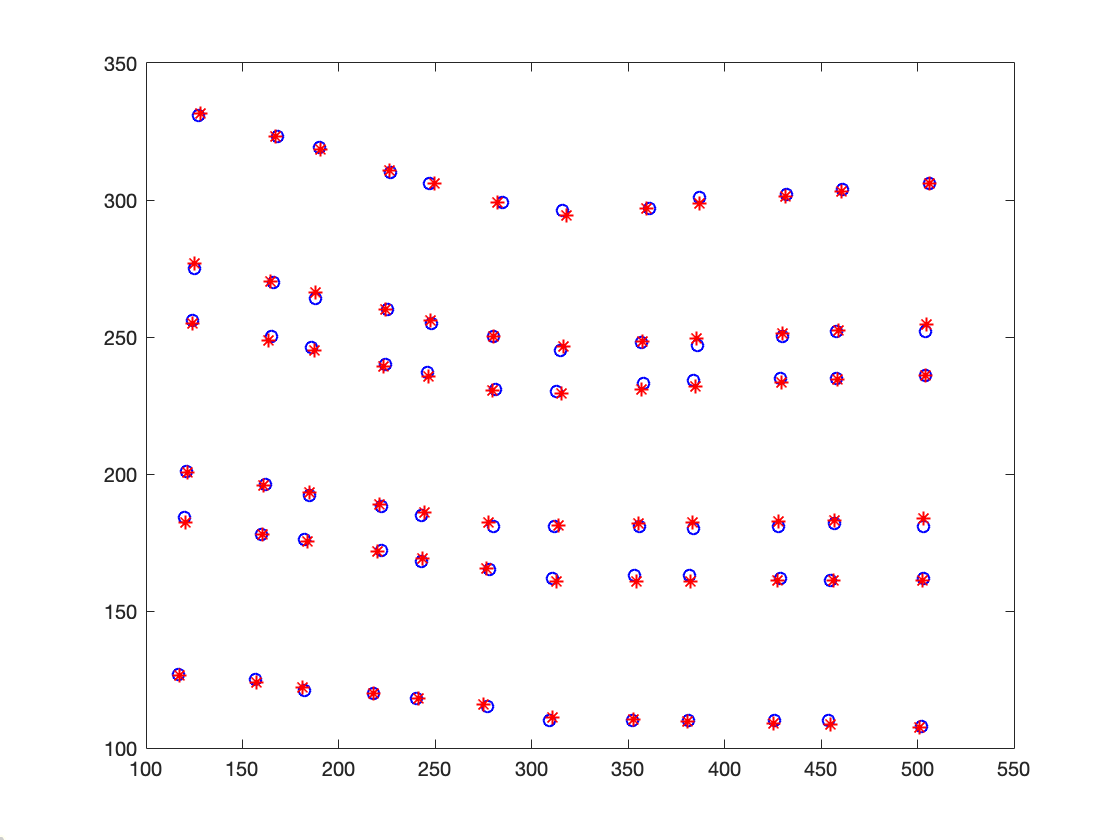
\includegraphics[scale=0.2]{Good.png}
\caption{points using good pairs}
\label{fig:label}
\centering
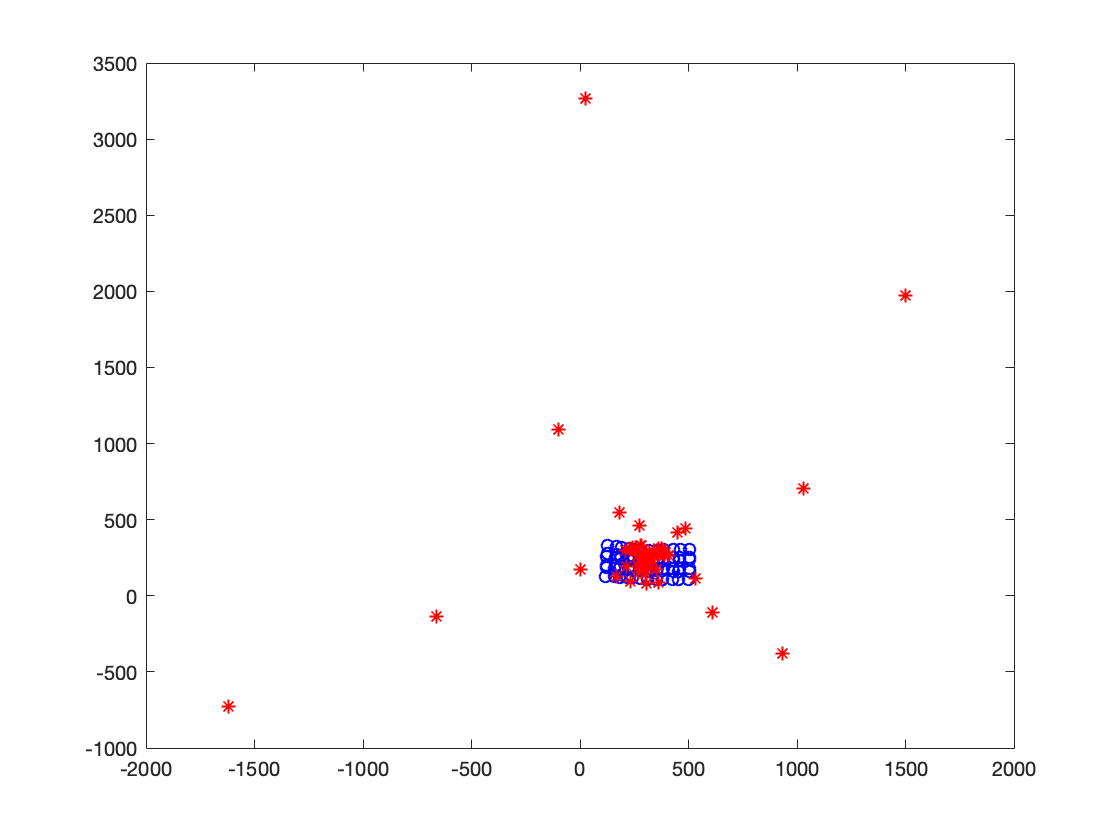
\includegraphics[scale=0.2]{Bad.png}
\caption{points using good pairs}
\label{fig:label}
\centering
\includegraphics[scale=0.2]{RANSAC.png}
\caption{points using good pairs}
\label{fig:label}
\end{figure}
In the figures above the blue circles are given 2D points and the red stars are 2D points from reprojection.
We can see from the intrinsic, extrinsic matrix and the figures that the results of using all the good pairs and using RANSAC are similar, and the result from bad pairs contains large errors. However the results from good pairs and RANSAC are not exactly the same. I think there are two major reasons.
\begin{enumerate}
\item Wrong $R,t$\\
The results of R and t via RANSAC are not consistent their signs vary as we choose different points to form the A matrix. That is because for equation AV=0, both P and -P satisfy the equation, which means that for W,-R,-t equation also is also satisfied.
\begin{equation}
\lambda_i\begin{bmatrix}c_i\\r_i\\1\end{bmatrix}=W\begin{bmatrix}-R&&-t\end{bmatrix}^{3\times4}\begin{bmatrix}X_i\\Y_i\\Z_i\\1\end{bmatrix}
\end{equation}
But this will cause a problem that the location of the points respect to the camera frame is behind the camera which is not possible in the real world.
To solve this, we need to decide the sign of , if it is positive, then the R and t are correct else we need to inverse the sign of R and t.
\item Noise in dataset\\
When using RANSAC method, some good points will be classified as outliers because of the noise when extracting feature points from image. Thus good 3D points whose coresponding 2D points have large noise will be classified as outliers. 
\end{enumerate}
\subsection*{Conclusion and summary}
In this project I used one of linear methods to calibrate a camera using given 3D/2D points. And I also applied RANSAC method to eliminate the error caused by bad 3D points. In conclusion, the result of using 72 good points and the result using RANSAC are similar and likely to be more correct. The bad points in dataset will ruin the result and make the calibration without RANSAC not useable at all. And the RANSAC method has a very good performance when the dataset contains bad data. After this project I learned how to use RANSAC method and SVD method for solving linear equations. Also I got a better knowledge of the details of the calibration algorithm. 
\newpage

\begin{thebibliography}{}  
\bibitem{ref1}Qiang Ji. RPI ECSE 6650 Computer Vision, Lecture Notes: Camera Calibration and Pose Estimation. URL:https://www.ecse.rpi.edu/~qji/CV/camera\_calibration\_pose\_estimation.pdf. Last visited on 2019/10/18.
\bibitem{ref2}Wikipedia contributors, "Random sample consensus"Wikipedia, the free encyclopedia, https://en.wikipedia.org/wiki/Random_sample_consensus(accessed October 18,2019).
\end{thebibliography}
\end{document}